\newpage
\customchapter{Product Overview}
The RV64I single-cycle RISC-V processor is a fundamental design that exemplifies simplicity and efficiency in modern computer architecture. This processor, which adheres to the RISC-V instruction set architecture (ISA), is characterized by its 64-bit width and single-cycle execution, where each instruction is completed in one clock cycle.\\
\vspace{\baselineskip}
\textbf{Fundamental design elements in RV64I are:}
\begin{itemize}
\item \textbf{The Program Counter (PC)} is a crucial component that holds the address of the next instruction to be executed in the sequence. On each clock cycle, the PC increments by 4 bytes, corresponding to the size of each instruction in the RISC-V architecture.
\item \textbf{Instruction Memory} is responsible for storing the program's instructions and supplying them to the processor. When the PC provides an address, the instruction memory retrieves the corresponding instruction and forwards it to the instruction decoder. This read-only memory is typically implemented as a ROM or a similar non-volatile storage, ensuring the integrity and availability of the program instructions throughout the execution cycle.
\item \textbf{The Instruction Decoder} plays a pivotal role in interpreting the binary instruction fetched from the instruction memory. It breaks down the instruction into its constituent parts, such as opcode, source registers, destination register, and immediate values. The decoder then generates the necessary control signals that guide the other components of the processor to perform the specified operation, whether it be an arithmetic calculation, memory access, or control flow alteration.
\item \textbf{The Register File} consists of a set of 32 general-purpose registers that store intermediate data and results during instruction execution. It includes two read ports and one write port, allowing two source operands to be read simultaneously and one result to be written back each cycle.
\item \textbf{The Arithmetic Logic Unit (ALU)} is the computational heart of the processor, responsible for performing arithmetic operations (such as addition, subtraction) and logical operations (such as AND, OR, XOR). The ALU receives its operands from the register file or immediate values decoded from the instruction and executes the operation specified by the control signals from the instruction decoder. The result is then either written back to a register or used for further processing.
\item \textbf{Data Memory} is used for reading from and writing to memory locations during load and store instructions. The memory address is calculated by the ALU and sent to the data memory along with the data to be stored (for store operations) or a request to retrieve data (for load operations). This allows the processor to interact with memory to access data beyond the limited capacity of the register file, enabling larger and more complex computations.
\item \textbf{The Control Unit} generates the necessary control signals based on the decoded instruction. These signals direct the operation of other components like the ALU, data memory, and register file. It determines the type of operation (arithmetic, logical, load, store, branch) and configures the processor’s pathways accordingly.
\end{itemize}
Our design is capable of executing memory-reference instructions load doubleword (ld) and store doubleword (sd), the arithmetic-logical instructions add, sub, and, and or, and the conditional branch instruction branch if equal (beq).\\
\vspace{\baselineskip}
\textbf{For every instruction, the first two steps are identical:}
\begin{itemize}
\item Send the program counter (PC) to the memory that contains the code and fetch the instruction from that memory.
\item Read one or two registers, using fields of the instruction to select the registers to read. For the ld instruction, we need to read only one register, but most other instructions require reading two registers.
\end{itemize}
After these two steps, the actions required to complete the instruction depend on the instruction class. The three instruction classes involved in this design are memory-reference, arithmetic-logical, and branches. All instruction classes use the arithmetic-logical unit (ALU) after reading the registers. The memory-reference instructions use the ALU for an address calculation, the arithmetic logical instructions for the operation execution, and conditional branches for the equality test. After using the ALU, the actions required to complete various instruction classes differ. A memory reference instruction will need to access the memory either to read data for a load or write data for a store. An arithmetic-logical or load instruction must write the data from the ALU or memory back into a register. Lastly, for a conditional branch instruction, we may need to change the next instruction address based on the comparison; otherwise, the PC should be incremented by four to get the address of the subsequent instruction.\\
\vspace{\baselineskip}
Below figure shows the high-level view of a RISC-V implementation, focusing on the various functional units and their interconnection along with the required multiplexors as well as control lines for the major functional units.
 \begin{figure}[H]
    \centering
    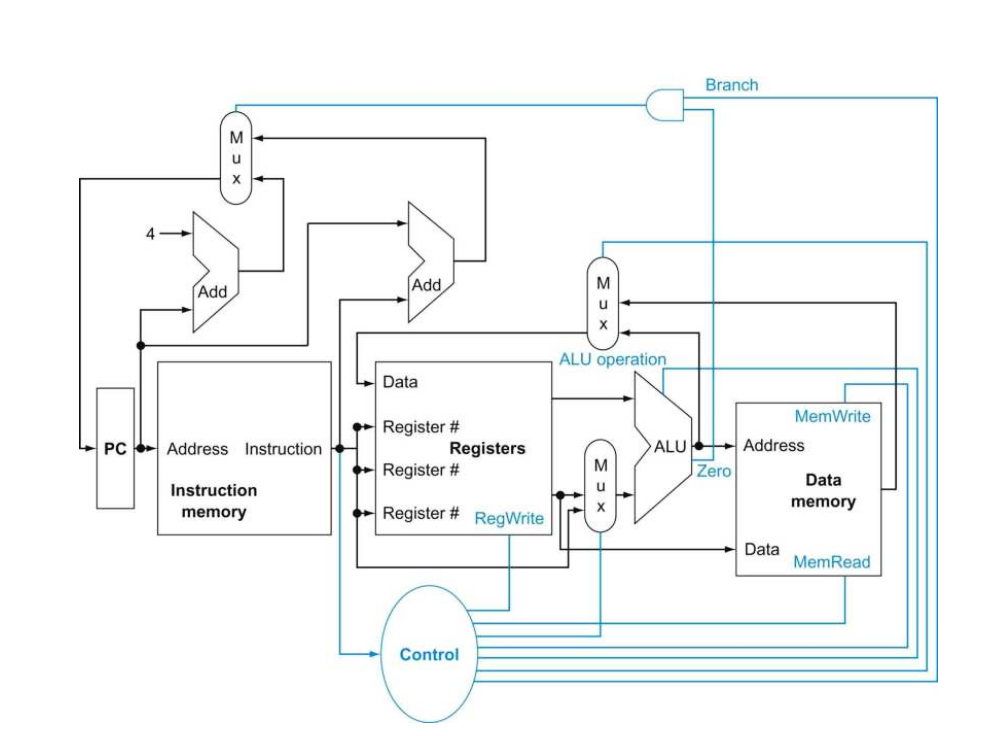
\includegraphics[width=0.8\linewidth]{Image/Abstract.png}
    \caption{Abstract view of RV64I}
    \label{fig:enter-label}
\end{figure}
All instructions start by using the program counter to supply the instruction address to the instruction memory. After the instruction is fetched, the register operands used by an instruction are specified by fields of that instruction. Once the register operands have been fetched, they can be operated on to compute a memory address (for a load or store), to compute an arithmetic result (for an integer arithmetic-logical instruction), or an equality check (for a branch). If the instruction is an arithmetic-logical instruction, the result from the ALU must be written to a register. If the operation is a load or store, the ALU result is used as an address to either store a value from the registers or load a value from memory into the registers. The result from the ALU or memory is written back into the register file. Branches require the use of the ALU output to determine the next instruction address, which comes either from the adder (where the PC and branch offset are summed) or from an adder that increments the current PC by four. The thick lines interconnecting the functional units represent buses, which consist of multiple signals. The arrows are used to guide the reader in knowing how information flows. Since signal lines may cross, we explicitly show when crossing lines are connected by the presence of a dot where the lines cross.\\
\vspace{\baselineskip}
The multiplexors are used to regulate the flow of the data to various design elements depending on the class of the instruction that is being executed. These multiplexors are controlled by various control signals decoded from the instruction itself. A detailed description of the instruction decoding, control signals, datapath and other necessary design elements will be given in detail in Chapter 6.